\chapter{Numerical results} \label{sec:numerical_results}

This chapter presents two sets of results concerning the subject of thermomechanical modeling of semi-crystalline polymers.
The first is adapted from \cite{vila-chaNumericalAssessmentPartitioned2023a} and pertains to the implicit partitioned solution of the thermomechanical model employing a elasto-plastic description for the material.
The nonlinear solvers available are compared and analysed according to their CPU time, memory use and ...
The second pertains to the implementation and validation of state of the art constitutive models for semi-crystalline polymers.


\section{Necking of a thermoelastoplastic circular bar}
     \label{sec:mech-driv-probl}

     The thermomemechanical problem under analysis consists of the thermally triggered necking of a circular bar, as initially reported in \cite{simo_associative_1992} and replicated in \cite{danowski_computational_2014}.
     The problem consists of a cylindrical bar of radius $r=\SI{6.413}{\milli\meter}$ and length $h=\SI{53.334}{\milli\meter}$ subject to a prescribed axial displacement $\bar{u}_{y}=\SI{8}{\milli\meter}$ at both ends during $t_s=\SI{8}{\second}$.
     The supports at the tips allow the contraction of the specimen.
     The bar is initially at room $T_{0}=T_{\infty}=\SI{293}{\kelvin}$ and is subject to heat transfer by convection at all boundaries, with a heat transfer coefficient $h_{c} = \SI{17.5e-3}{\newton\milli\meter^{-1}\second^{-1}\kelvin^{-1}}$.
     The material is modeled by the constitutive model proposed by Simo and Miehe \citep{simo_associative_1992}, and the material properties are given in Table~\ref{tab:matpropsnecking}.
     %
     \begin{table}
       \centering
       \caption{Material properties and initial and boundary conditions for the problem concerning the necking of a thermoplastic circular bar.}
       \label{tab:matpropsnecking}
       \begin{tabular}{lccS[exponent-mode=engineering]}
         \hline\hline
         \multicolumn{3}{l}{\textbf{Material Properties}} & {\vphantom{\Big |}Effective value}\\
         \hline
         \vphantom{\Big |}Density & \(\rho\) & (\si{\newton\second^2\milli\meter^{-4}}) & 7.8e-9\\
         \vphantom{\Big |}Bulk modulus & \(\kappa\) & (\si{\newton\milli\meter^{-2}}) & 164206\\
         \vphantom{\Big |}Shear modulus & \(\mu\) & (\si{\newton\milli\meter^{-2}}) & 801938\\
         \vphantom{\Big |}Conductivity & \(k\) & (\si{\newton\second^{-1}\kelvin^{-1}}) & 45\\
         \vphantom{\Big |}Heat capacity & \(C_{\mathbf F}\) & (\si{\milli\meter^2\second^{-2}\kelvin^{-1}}) & 460e6\\
         \vphantom{\Big |}Coefficient of thermal expansion & \(\alpha_T\) & (\si{\kelvin^{-1}}) & 10e-6\\
         \vphantom{\Big |}Dissipation factor & \(\chi\) & (-) & 900e-3\\
         \vphantom{\Big |}Initial yield stress at \(T_0\) & \(\sigma_{y,0}\) & (\si{\newton\milli\meter^{-2}}) & 450\\
         \vphantom{\Big |}Linear hardening coefficient at \(T_0\) & \(H\) & (\si{\newton\milli\meter^{-2}}) & 129.24\\
         \vphantom{\Big |}Saturation exponent & \(\delta\) & (-) & 16.93\\
         \vphantom{\Big |}Saturation yield stress at \(T_0\) & \(\sigma_{y,\infty}\) & (\si{\newton\milli\meter^{-2}}) & 715\\
         \vphantom{\Big |}Thermal softening parameter (\(\sigma_{y,0}\)) & \(\w_0\) & (\si{\kelvin^{-1}}) & 2e-3\\
         \vphantom{\Big |}Thermal softening parameter (\(\sigma_{u,\infty}, H\)) & \(\w_h\) & (\si{\kelvin^{-1}}) & 2e-3\\
         \hline
         \multicolumn{3}{l}{\textbf{Boundary Conditions}\vphantom{\Big |}} & \\\hline
         \vphantom{\Big |}Radius of the cylindrical bar & \(r\) & (\si{\milli\meter}) & 6.413\\
         \vphantom{\Big |}Length of the cylindrical bar & \(h\) & (\si{\milli\meter}) & 53.334\\
         \vphantom{\Big |}Maximum displacement at both ends & \(\bar u_y\) & (\si{\milli\meter}) & 8\\
         \vphantom{\Big |}Time to maximum displacement & \(t\) & (\si{\second}) & 8\\
         \vphantom{\Big |}Heat transfer coefficient & \(h_c\) & (\si{\newton\milli\meter^{-1}\kelvin^{-1}}) & 17.5e-3\\
         % \multicolumn{3}{l}{\vphantom{\Big |}All mechanical degrees of freedom fixed in the \(y\)- and \(z\)-directions.}\\
         \hline
         \multicolumn{3}{l}{\textbf{Initial Conditions}\vphantom{\Big |}} & \\\hline
         Initial temperature & \(T_0\) & (\si{\kelvin}) & {293}\\
         \hline
         \multicolumn{3}{l}{\textbf{Reference value} \vphantom{\Big |}} & \\\hline
         \vphantom{\Big |}Temperature at outer radius (\(r\)) & & (\si{\kelvin}) & \\
         \vphantom{\Big |}Longitudinal reaction forces & & (\si{\newton}) & \\
         \hline\hline
       \end{tabular}
     \end{table}

     %
     This classical benchmark in isothermal elastoplasticity renders a bifurcation problem where a geometric imperfection triggers the necking phenomenon.
     In the thermomechanical version, the combination of the plastic dissipation in the bulk material and the heat transfer at the boundaries produce a temperature field that becomes progressively more heterogeneous during the loading.
     With growing elongation, the temperature rise in the center of the bar increases relative to the exterior boundary and triggers the necking as a result, even for a geometrically perfect setup.

     The problem is analyzed using two-dimensional axisymmetric QUAD4-FBAR elements \citep{de_souza_neto_design_1996} for the mechanical problem and QUAD4 elements for the thermal problem.
     Figure~\ref{fig:necking} illustrates the problem setup, the finite element mesh employed in the 2D simulations, and distinct stages of deformation and temperature field during the prescribed elongation, evidencing the significant necking of the bar.
     %
     \begin{figure}[p]
       \centering
       % \def\svgwidth{1.0\linewidth}
       % \footnotesize
       % \input{figures/necking.pdf_tex}
       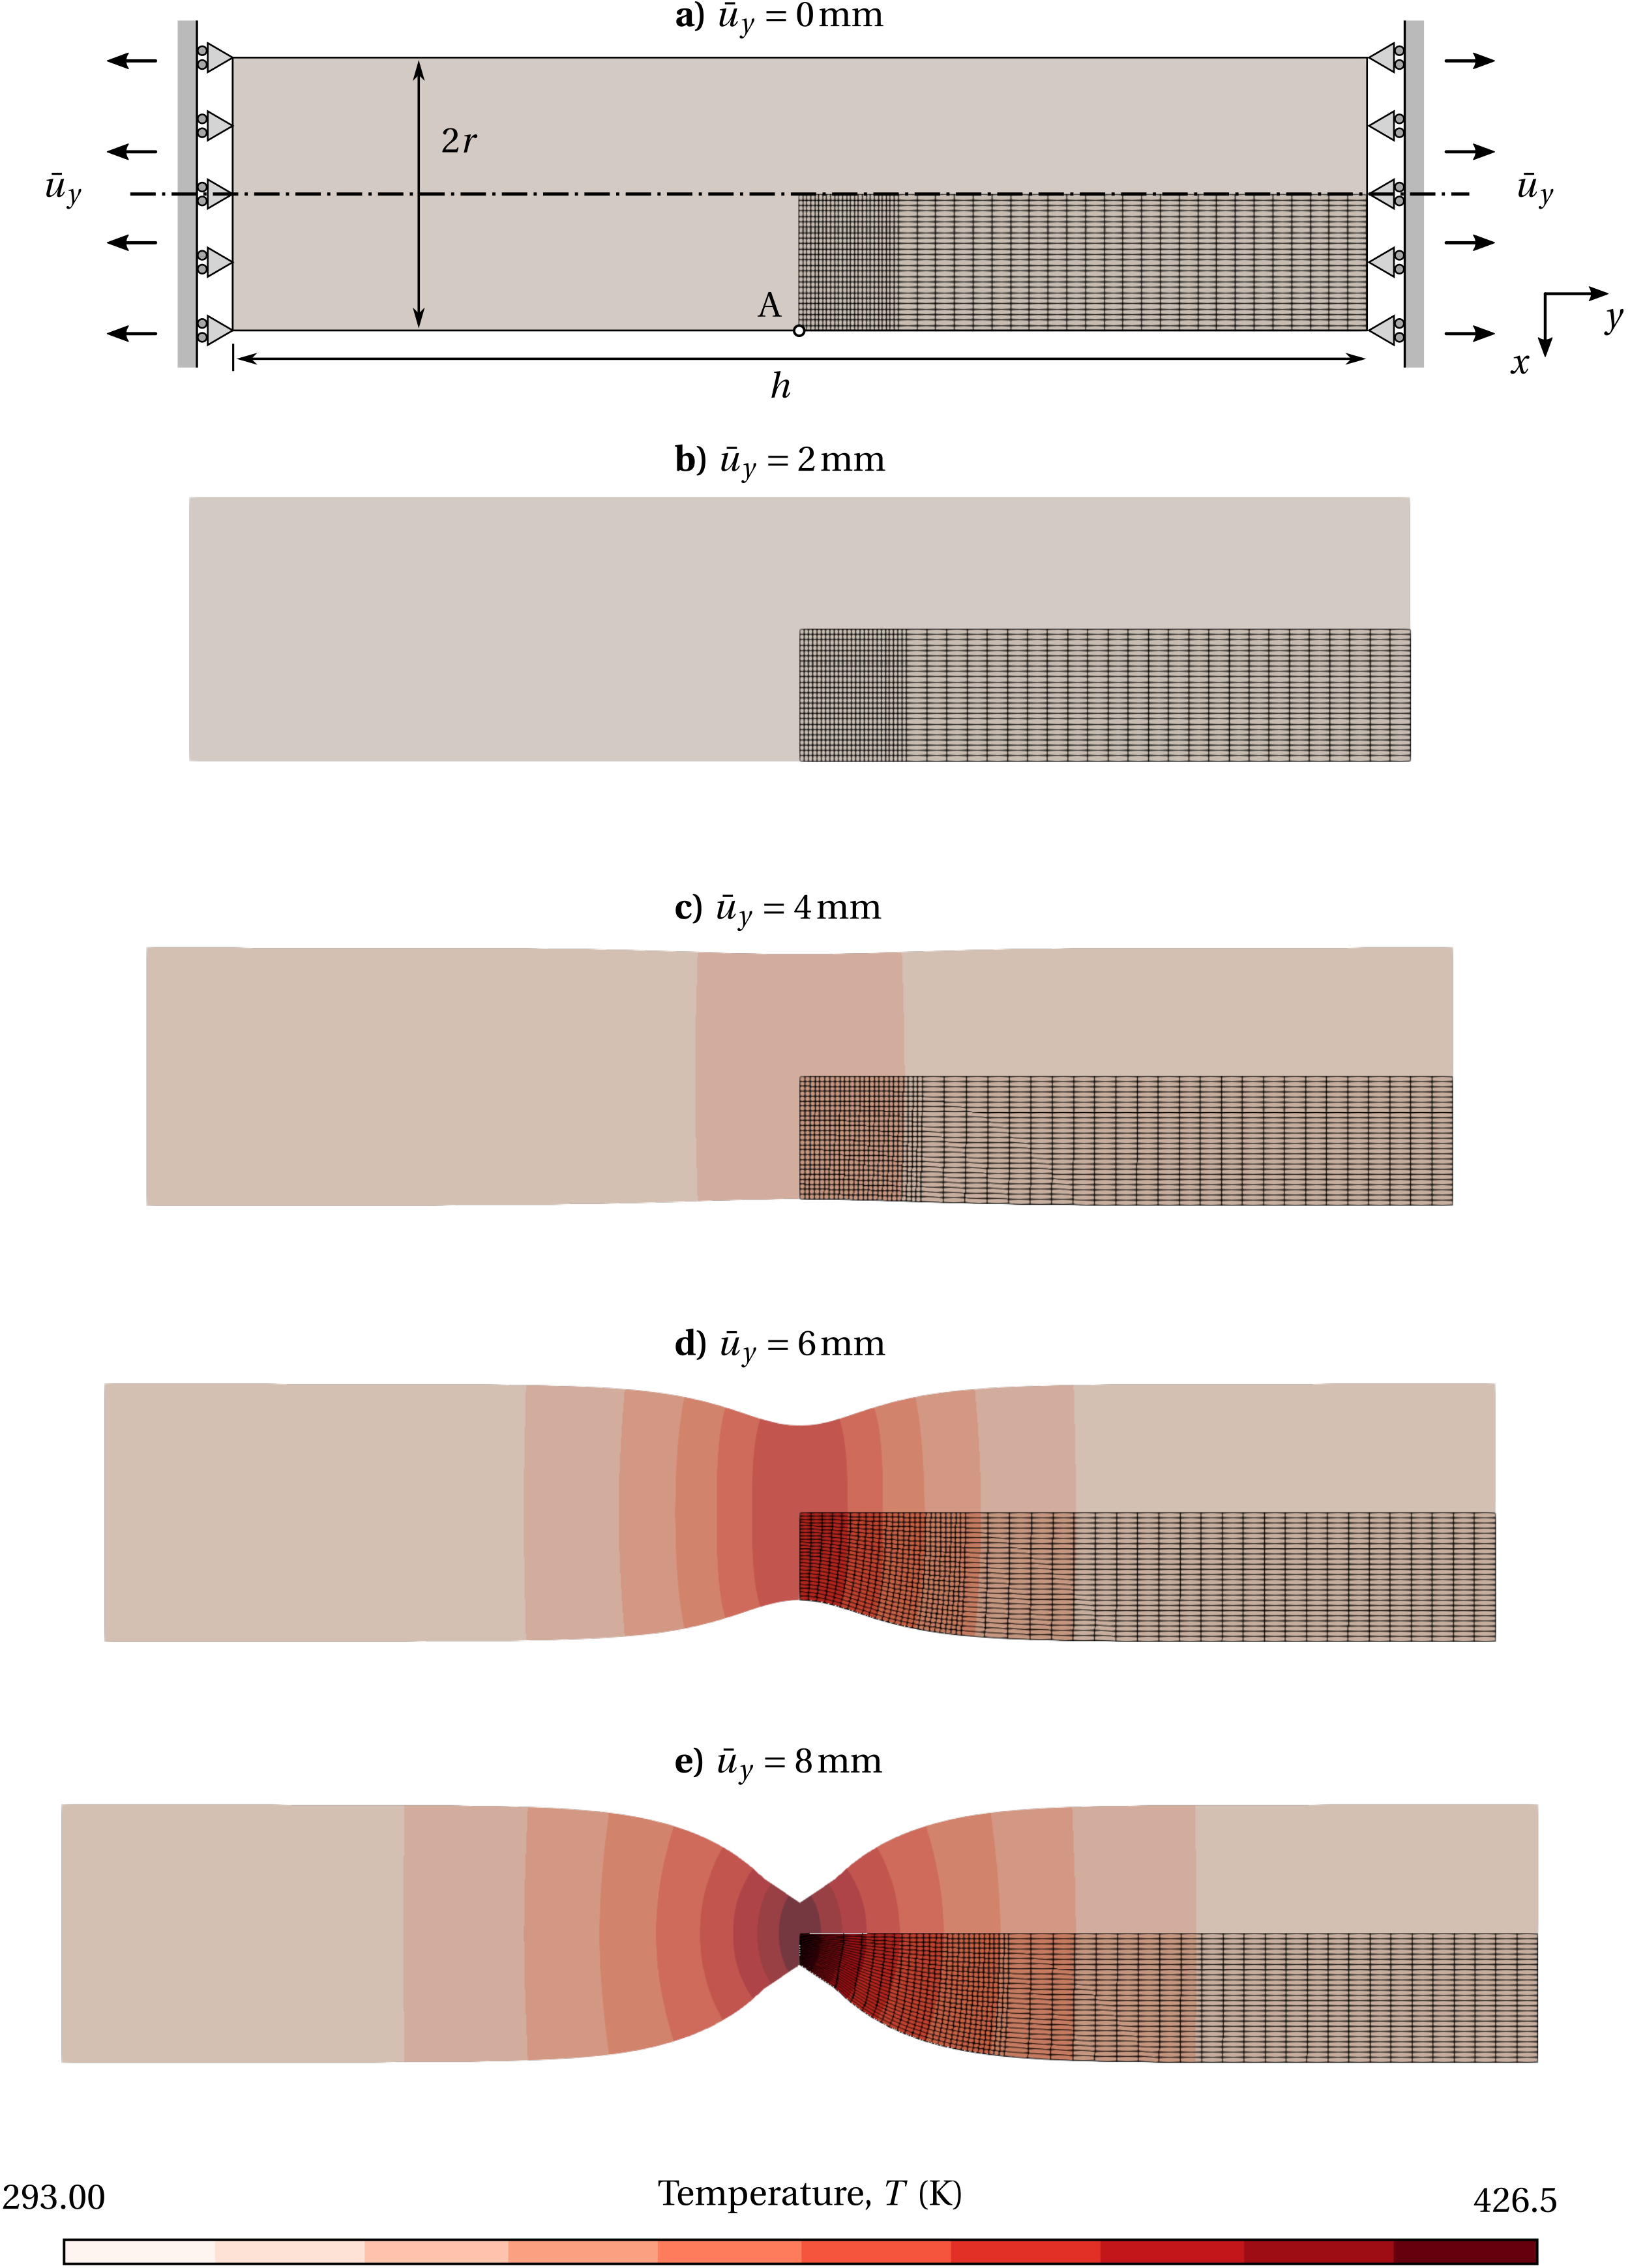
\includegraphics[width=0.9\linewidth]{figures/necking3.png}
       \caption{Deformation of the thermally triggered necking of a thermoplastic circular bar and temperature field stages during the loading and axisymmetric finite element mesh. The results are obtained with QUAD4-FBAR elements for the mechanical problem and QUAD4 elements for the thermal problem, non-adiabatic boundary conditions, the inconsistent mechanical dissipation formulation, and the Fourier law based on constant $k_{0}$.}
       \label{fig:necking}
     \end{figure}
     %
     Only one-quarter of the specimen is simulated, resulting in a finite element mesh with 1326 nodes and 1250 elements.
     Unless otherwise stated, this mesh is employed in the following analyses.
     The load is applied in a total of 80 equal magnitude increments and considering a constant incremental time step of \(\Delta t = \SI{0.1}{\second}\).
     A quasi-static solution is computed for the mechanical problem using a backward Euler integration. The transient temperature field is integrated with the generalised-$\alpha$ method with $\rho_{\infty, T}=1.0$.

     \subsubsection{Validation of the numerical results}

     The reaction force at the supports and the neck surface temperature at point A are compared to results found in the literature to validate the computationally implemented solution procedure, as shown in Figure \ref{fig:necking}.
     The analysis's reference data may be found in \cite{simo_associative_1992}.
     It should be noted that key distinctions between the current work and the reference lead to slightly different outcomes.
     Regarding the heat conduction law employed in each contribution, although the large deformation version of the Fourier law is adopted in both works, Simo and Miehe \citep{simo_associative_1992} considered the spatial thermal conductivity, $k$, as a fixed material parameter.
     In the present work, the material thermal conductivity, $k_{0}$, is interpreted as the fixed material parameter.
     In addition, Simo and Miehe \citep{simo_associative_1992} solved the coupled problem using an explicit scheme, while in the present work, an implicit schemes is considered.
     Lastly, regarding  spatial discretisation, Simo and Miehe \citep{simo_associative_1992} employed mixed displacement-pressure QUAD8 elements.

     The evolution of the reaction force and the neck surface temperature as a function of the prescribed displacement are shown in Figure~\ref{fig:necking_force_temperature_coupled_quad4fbar}.
     \begin{figure}[!hbtp]
       \centering
       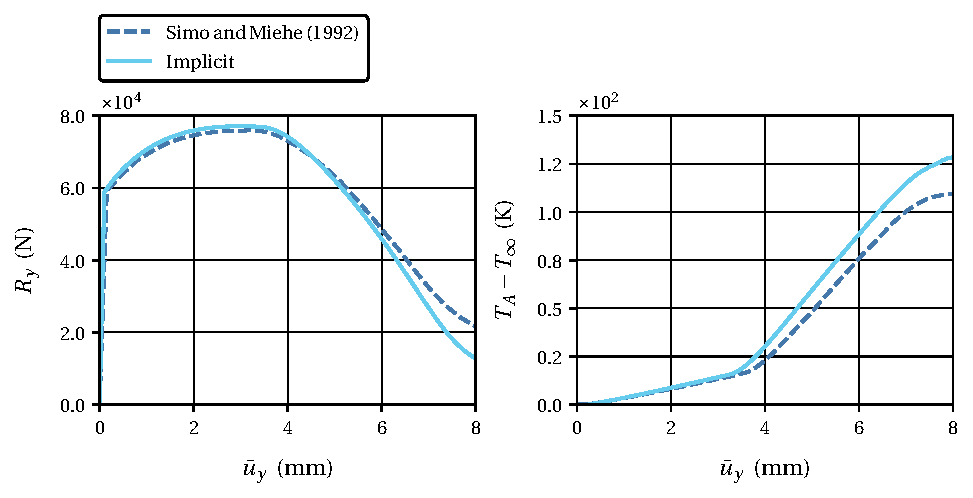
\includegraphics[width=.85\textwidth]{necking_force_temperature_coupled_quad4fbar}
       \caption{Evolution of the reaction force at the tips of the bar and the neck surface temperature with the prescribed displacement using QUAD4-FBAR elements for the mechanical problem and QUAD4 elements for the thermal problem.}
       \label{fig:necking_force_temperature_coupled_quad4fbar}
     \end{figure}
     %
     From a physical point of view, the reaction forces show that the simulation occurs almost entirely in the elastoplastic regime.
     As previously mentioned, necking is automatically triggered, resulting in a significant reduction of the reaction force starting at approximately $\bar{u}_{y}=\SI{4}{\milli\meter}$, followed by a steep temperature rise due to the higher plastic dissipation around the necking region.

     Inspecting Figure~\ref{fig:necking_force_temperature_coupled_quad4fbar} from a validation perspective, the numerical results show a reasonable agreement with the literature.
     Regarding the reaction force at the supports, there is a good agreement for most of the displacement range examined, except for the largest values, where some discrepancy is be observed.
     There are larger disparities in the neck surface temperature at point A, with noticeable differences for displacements larger than \(\bar{u}_y\approx\SI{3.5}{\milli\meter}\).
     However, the differences previously mentioned between the modeling approaches adopted in the present work and in \cite{simo_associative_1992} offer sufficient justification for the differences observed.

     \subsubsection{Comparison of implicit solution methods}

     As in Section~\ref{sec:comparison_thick_cylinder}, the chosen set of implicit methods for the solution of thermomechanical problems are compared, this time considering a thermoplastic constitutive behavior.
     The maximum displacement at both ends is restricted to \SI{5}{\milli\meter}, applied in \SI{5}{\second} in 100 increments (\(\Delta t = \SI{0.05}{\second}\)) to prevent an excessive elongation of the elements in the finite element simulation.
     The coupling strength is correlated with the value of thermal softening parameters \(w_0\) and \(w_h\), set to be equal.
     Its effect on the implicit solution of the problem is an increased number of nonlinear iterations to solve the problem, as is illustrated in Figure~\ref{fig:necking_single_iter_diff_w_0_n_iter_time_quad4fbar_pred}, although with less prominence than in the previous problem (Figure~\ref{fig:thick_cylinder_single_iter_n_iter_diff_coeff_exp_time_quad4fbar_pred}).
     It depicts the number of nonlinear iterations needed to solve the coupled problem at each time step and the corresponding total number of residual evaluations as a function of the thermal expansion coefficient for the fixed-point method in the solution of the necking of a circular bar with \(w_0=w_h\in\{\SI{2e-3}{},\, \SI{4.89e-3}{},\, \SI{1e-2}{}\}\,\si{\kelvin^{-1}}\).
     A higher total number of nonlinear iterations per time step is necessary to solve the problem as \(w_0\) and \(w_h\) increase, corresponding to a taller and broader peak in the number of iterations needed to solve the problem per time step.
     The coupling strength is the most intense when the necking begins, which occurs at different moments as \(w_0\) and \(w_h\) vary.
     This peak is the main contributor to the difference in the total number of iterations taken to solve each problem with different softening parameters.
     Once again, the improvement in the efficiency achieved by the implicit methods under analysis is obtained by decreasing the number of nonlinear iterations needed to solve the problem when the coupling is the most challenging, as can be concluded from Figure~\ref{fig:necking_comparison_best_n_iter_time_quad4fbar_pred}.
     It shows the number of nonlinear iterations needed to solve the coupled problem at each time step and the total number of residual evaluations as a function of the thermal expansion coefficient for several implicit methods in the solution of the necking of a circular bar with \(w_0=w_h=\SI{1e-2}{\kelvin^{-1}}\).
     On the other hand, when the coupling is not as demanding, the difference between the different methods is hardly noticeable.

     \begin{figure}[htbp]
       \centering
       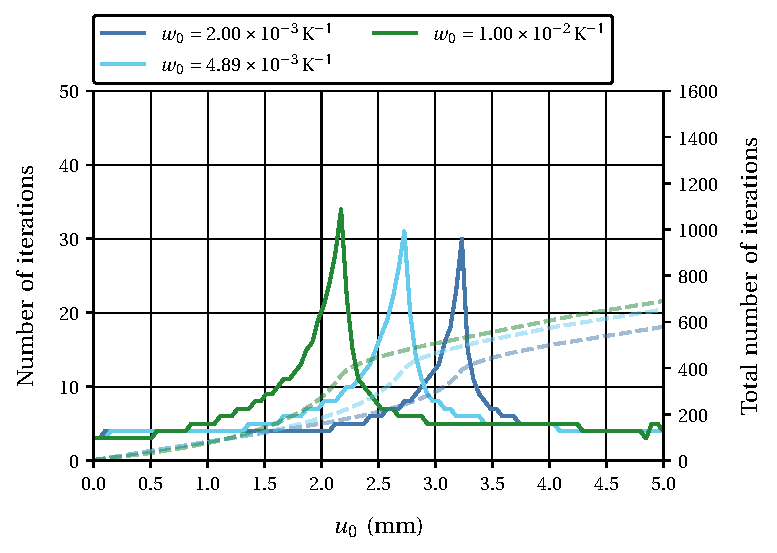
\includegraphics[width=.7\textwidth]{necking_single_iter_diff_w_0_n_iter_time_quad4fbar_pred}
       \caption{Number of nonlinear iterations needed to solve the coupled problem at each time step (continuous) and the total number of residual evaluations (dashed) as a function of the thermal expansion coefficient for the fixed-point method in the solution of the necking of a circular bar with \(w_0=w_h\in\{\num{2e-3},\ \num{4.89e-3},\ \num{1e-2}\}\si{\kelvin^{-1}}\).}
       \label{fig:necking_single_iter_diff_w_0_n_iter_time_quad4fbar_pred}
     \end{figure}

     \begin{figure}[!hbtp]
       \centering
       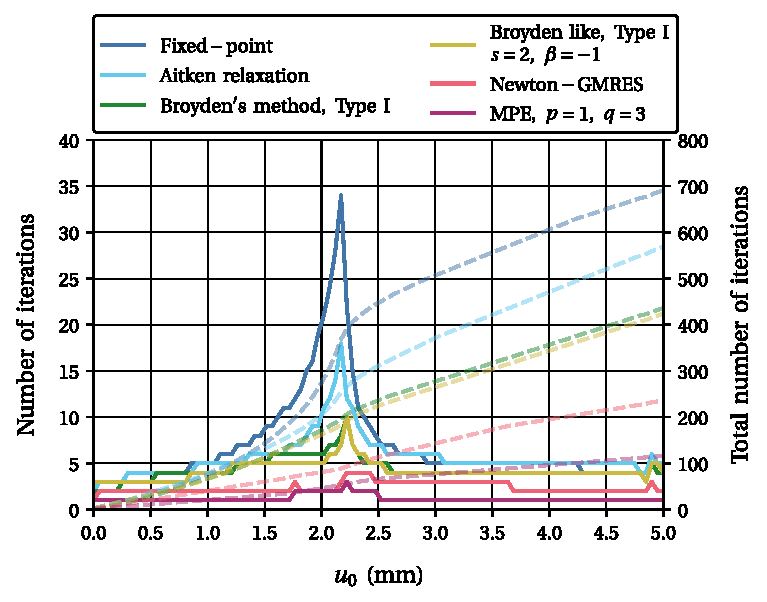
\includegraphics[width=.7\textwidth]{necking_comparison_best_n_iter_time_quad4fbar_pred}
       \caption{Number of nonlinear iterations needed to solve the coupled problem at each time step (continuous) and the total number of residual evaluations (dashed) as a function of the thermal expansion coefficient for several implicit methods in the solution of the necking of a circular bar with \(w_0=w_h=\SI{1e-2}{\kelvin^{-1}}\).}
       \label{fig:necking_comparison_best_n_iter_time_quad4fbar_pred}
     \end{figure}


     It is pointed out that what is depticted in Figures~\ref{fig:thick_cylinder_single_iter_n_iter_diff_coeff_exp_time_quad4fbar_pred} and \ref{fig:thick_cylinder_comparison_best_n_iter_time_quad4fbar_pred} is the number of nonlinear and not the number of residual evaluation per time step.
     Thus, for comparisons concerning the computational efficiency of the different methods under analysis, the information shown in
     Figure~\ref{fig:necking_comparison_best_cpu_time_n_iter_coupl_strength_quad4fbar_pred} is more appropriate, as it displays the total CPU time in seconds and the total number of residual evaluations as a function of the thermal softening parameters.
     As before, the best performing methods are the Broyden-like methods, whose performance is very similar.
     They are followed by the Aitken relaxation and the MPE in cycling mode, also displaying a comparable efficiency.
     The Newton-GMRES method is the worse performing method considered, being around 20\% slower than the Broyden-like methods and roughly on par with the fixed-point method.
     Moreover, it fails to converge for \(w_0=w_h=\SI{2e-3}{\kelvin^{-1}}\).
     The comments in Section~\ref{sec:comparison_thick_cylinder} regarding memory requirements and ease of implementation also apply here.
     Table~\ref{tab:necking_res_cpu_nr_func_best} summarizes all the results previously discussed regarding the computational time each implicit method takes and the number of residual evaluations.

     \begin{figure}[!hbtp]
       \centering
       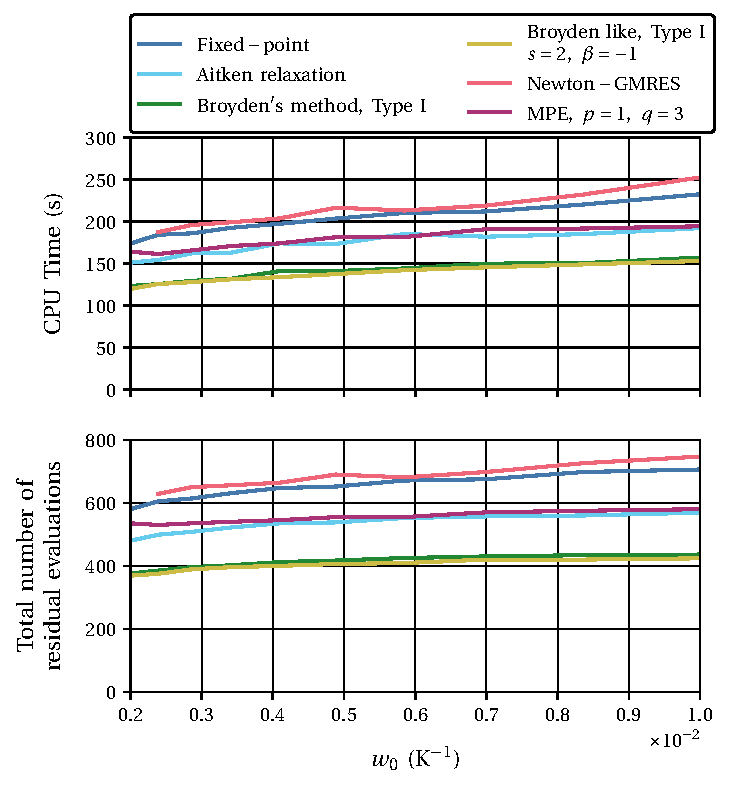
\includegraphics[width=.7\textwidth]{necking_comparison_best_cpu_time_n_iter_coupl_strength_quad4fbar_pred}
       \caption{Total CPU time in seconds and the total number of residual evaluations as a function of the thermal softening parameters \(w_0=w_h\) in the solution of the necking of a thermoplastic circular bar with \(w_0=w_h=\SIrange{2e-3}{1e-2}{\kelvin^{-1}}\).}
       \label{fig:necking_comparison_best_cpu_time_n_iter_coupl_strength_quad4fbar_pred}
     \end{figure}

     \begin{table}[hbtp]
       \centering
       \caption{Total CPU time in seconds and the total number of residual evaluations as a function of the thermal softening parameters \(w_0=w_h\) in the solution of the necking of a thermoplastic circular bar with \(w_0=w_h\in\{\num{2e-3},\ \num{4.89e-3},\ \num{1e-2}\}\si{\kelvin^{-1}}\). The best performances are highlighted in gray.}
       \label{tab:necking_res_cpu_nr_func_best}
       % \setlength{\tabcolsep}{3pt}
       \begin{tabular}
         {l
         S[round-mode=places, round-precision=2, table-format = 1.2e1]
         S[round-mode=places, round-precision=2, table-format = 1.2e1]
         S[round-mode=places, round-precision=2, table-format = 1.2e1]
         S[round-mode=places, round-precision=0, exponent-mode=fixed, fixed-exponent=0, table-number-alignment = center, table-format = 4.0]
         S[round-mode=places, round-precision=0, exponent-mode=fixed, fixed-exponent=0, table-number-alignment = center, table-format = 4.0]
         S[round-mode=places, round-precision=0, exponent-mode=fixed, fixed-exponent=0, table-number-alignment = center, table-format = 4.0] }
         \vphantom{\Big \vert}&  \multicolumn{3}{c}{CPU Time (\si{\second})} & \multicolumn{3}{c}{Nr Residual Evaluations} \\
         \cmidrule(lr){2-4}\cmidrule(lr){5-7}
         \vphantom{\Big \vert}\makecell[c]{$w_0$\\ (\SI[exponent-mode=input]{1e-3}{\kelvin^{-1}})} & {2} & {4.89} & {10} & {2} & {4.89} & {10}\\
         \hline\hline
         % \vphantom{\Big \vert} AITK  & 1.51000e+02 & 1.73300e+02 & 1.92100e+02 & 4.80000e+02 & 5.38000e+02 & 5.69000e+02\\
         % \vphantom{\Big \vert} BRDI  & 1.23200e+02 & 1.41000e+02 & 1.57000e+02 & 3.76000e+02 & 4.17000e+02 & 4.36000e+02\\
         % \vphantom{\Big \vert} BRDI2  & \cellcolor{lightgray} 1.19700e+02 & \cellcolor{lightgray}1.37400e+02 & \cellcolor{lightgray}1.53000e+02 & \cellcolor{lightgray}3.69000e+02 & \cellcolor{lightgray}4.06000e+02 & \cellcolor{lightgray}4.24000e+02\\
         % \vphantom{\Big \vert} NEWT  & 9.54200e+01 & 2.16400e+02 & 2.52400e+02 & 4.40000e+02 & 7.90000e+02 & 8.47000e+02\\
         % \vphantom{\Big \vert} MPE  & 1.64100e+02 & 1.81300e+02 & 1.94300e+02 & 5.35000e+02 & 5.55000e+02 & 5.80000e+02\\


         \vphantom{\Big \vert} FXPT  & 1.73800e+02 & 2.03500e+02 & 2.32400e+02 & 5.80000e+02 & 6.52000e+02 & 7.06000e+02\\
         \vphantom{\Big \vert} AITK  & 1.51000e+02 & 1.73300e+02 & 1.92100e+02 & 4.80000e+02 & 5.38000e+02 & 5.69000e+02\\
         \vphantom{\Big \vert} BRDI  & 1.23200e+02 & 1.41000e+02 & 1.57000e+02 & 3.76000e+02 & 4.17000e+02 & 4.36000e+02\\
         \vphantom{\Big \vert} BRDI2  & \cellcolor{lightgray}1.19700e+02 & \cellcolor{lightgray}1.37400e+02 & \cellcolor{lightgray}1.53000e+02 & \cellcolor{lightgray}3.69000e+02 & \cellcolor{lightgray}4.06000e+02 & \cellcolor{lightgray}4.24000e+02\\
         \vphantom{\Big \vert} NEWT  & NC & 2.16400e+02 & 2.52400e+02 & NC & 6.90000e+02 & 7.47000e+02\\
         \vphantom{\Big \vert} MPE  & 1.64100e+02 & 1.81300e+02 & 1.94300e+02 & 5.35000e+02 & 5.55000e+02 & 5.80000e+02\\

         \hline\hline
       \end{tabular}
     \end{table}

     \subsubsection{Effect of predictors}

     Figure~\ref{fig:necking_comparison_best_pred_total_iters_coupl_strength_quad4fbar_pred} presents the effect of employing a linear or quadratic predictor on the number of residual evaluations needed to fully solve the thermomechanical problem under analysis as a function of the softening parameters.
     All methods improve using the polynomial predictors, with the best effects being achieved using the quadratic predictor.
     The decrease in residual evaluations is around 30\% for all methods using the quadratic predictor at \(w_0=w_h=\SI{1e-2}{\kelvin^{-1}}\) corresponding to the strongest coupling, except for the MPE.
     The polynomial vector extrapolation method displays a much smaller increase in efficiency from the polynomial predictors considered.
     This is again because using a predictor the problem is solved at most time steps in a single nonlinear iterations, requiring each five residual evaluations.
     Thus 100 increments lead to 500 residual evalutions for the whole simulation if each time step is solved in a single nonlinear iteration.
     Further considerations previously mentioned in Section~\ref{sec:effect_pred_thick} also apply.
     Finally, the use of predictors allows the Newton-GMRES method to converge for \(w_0=w_h=\SI{2e-3}{\kelvin^{-1}}\).

     \begin{figure}[!hbtp]
       \centering
       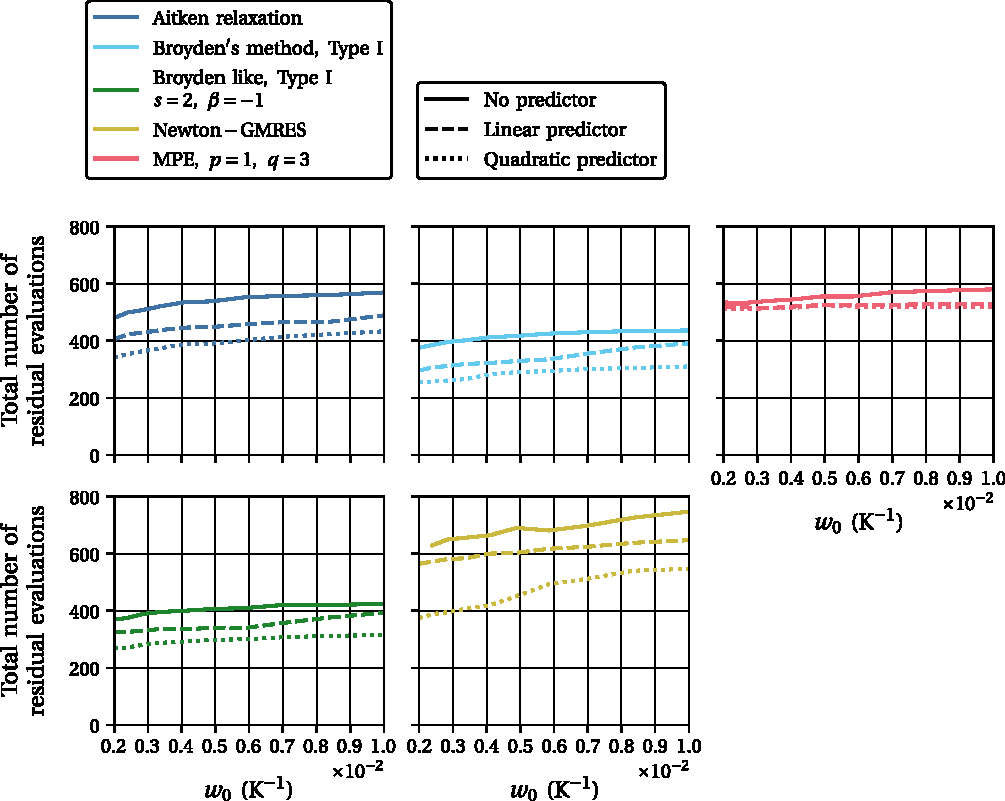
\includegraphics[width=.7\textwidth]{necking_comparison_best_pred_total_iters_coupl_strength_quad4fbar_pred}
       \caption{Total number of iterations as a function of the thermal softening parameters \(w_0=w_h\) using a linear, a quadratic, and no predictor in the solution of the necking of a circular bar with \(w_0=w_h=\SIrange{2e-3}{1e-2}{\kelvin^{-1}}\).}
       \label{fig:necking_comparison_best_pred_total_iters_coupl_strength_quad4fbar_pred}
     \end{figure}

\section{State of the art in semi-crystalline polymer modeling}

This section analyses two state-of-the-art constitutive models for semi-crystalline polymers.
The first model is described in \cite{haoUnifiedAmorphousCrystalline2022} and is applicable to polymer plastics in general, neglecting to consider the bulk crystallinity of the polymer excplicitly.
The second model can be found in \cite{abdul-hameedTwophaseHyperelasticviscoplasticConstitutive2014} and considers the crystallinity of the polymer explicitly, attempting to describe the polymer at different cyrstallinities with only one set of material parameters.

\paragraph{Computational framework}
The solution of the thermomechanical problem is achieved employing an approach described thorougly in \cite{bergstromMechanicsSolidPolymers2015} and \cite{alvesFastOptimizationbasedParameter2022}, whose \verb|Python| implementation is available in-house.
It is restrcited to displacement-driven uniaxial loading, traction or compression, and it achieves the solution of the mechanical problem through a minimization procedure.
In each time step the axial stretch is prescribed and the transversal stretches are obtained as those leading to a minimum in the transversal stresses.
This minimum should be zero as the boundary condition on the laterial surfaces corresponds to a free surface.
Accordingly, it is implicitly assumed that the response is homogeneous, which allows for comparisons solely with experimental results where the intrinsic response of the material is shown, free of size effects.

Regarding the thermal field, its inclusion is restricted to the isothermic and adiabatic cases.
The former coincides with a strain rate sufficiently slow so that the heat generated from the deformation is easily offloaded to the environment, keeping the temperature constant.
The latter corresponds to a strain rate so fast that no energy is exchanged with the environment during loading, approaching an adiabatic condition.
Arruda et al. \citep{arrudaEffectsStrainRate1995} employ the dimensionless number defined as $\tau_\text{therm} = t_\text{test}/t_d$ to probe how appropriate either of these assumptions is.
$t_\text{test}$ is defined as the test time to reach the true strain of $-1.0$ (in compression), and $t_d$ is thermal diffusion time of the speciment, which may be approximated as
\begin{equation}
  t_d \approx \frac{L^2}{2(k/\rho C_\mathbf{F})},
\end{equation}
where $L$ is a characteristic dimension of the specimen from the center of the deforming region to the nearest heat sink.
If $\tau_\text{therm} \ll 1$, it is safe to assume an adiabatic evolution, however if $\tau_\text{therm}\gg 1$, the experiment progresses isothermically.
$\tau_\text{therm}\approx 1$ points to  a coupled problem, in the sense that some heat is removed from the specimen as the experiment progresses, without however preventing an increase in temperature.

\colorbox{BrickRed}{How isothermic and adabiatic in practice?}

\subsection{\cite{haoUnifiedAmorphousCrystalline2022}}

Following the description in \cite{haoUnifiedAmorphousCrystalline2022}, the experimental results employed for validation are those of Khan and Farrokh \citep{khanThermomechanicalResponseNylon2006} obtained during the uniaxial compression of nylon 101 at a constant strain rate.
The material is modeled by the constitutive model proposed by Hao et al. \citep{haoUnifiedAmorphousCrystalline2022}, and the material properties are given in Table~\ref{tab:mat_prop_hao}.
%
\begin{table}[htbp]
  \centering
  \caption{Material properties and initial conditions for the uniaxial compression of nylon 101.}
  \label{tab:mat_prop_hao}
  \begin{tabular}{lccS[exponent-mode=engineering]}
    \hline\hline
    \multicolumn{3}{l}{\textbf{Material Properties}} & {\vphantom{\Big |}Effective value}\\
    \hline
    \vphantom{\Big |}Density & \(\rho\) & (\si{\newton\second^2\milli\meter^{-4}}) & 1.150e-9\\
    \vphantom{\Big |}Young modulus at $T_\text{ref}$ & \(E_{a,\text{ref}}\) & (\si{\newton\milli\meter^{-2}}) & 3.01e3\\
    \vphantom{\Big |}Reference temperature & \(T_\text{ref}\) & (\si{\kelvin}) & 295\\
    \vphantom{\Big |}Temperature dependence coefficient & \(\beta\) & (-) & 0.0037\\
    \vphantom{\Big |}Poisson's coefficient & \(\nu_I\) & (-) & 0.39\\
    \vphantom{\Big |}Heat capacity & \(C_{\mathbf F}\) & (\si{\milli\meter^2\second^{-2}\kelvin^{-1}}) & 1.500e6\\
    \vphantom{\Big |}Athermal peak strength & \(s_1\) & (\si{\mega\pascal}) & 140\\
    \vphantom{\Big |}First saturation strength & \(s_2\) & (\si{\mega\pascal}) & 138\\
    \vphantom{\Big |}Second saturation strength & \(s_3\) & (\si{\mega\pascal}) & 183\\
    \vphantom{\Big |}Pre-peak hardening & \(h_1\) & (\si{\mega\pascal}) & 627e1\\
    \vphantom{\Big |}Post-peak softening & \(h_2\) & (\si{\mega\pascal}) & 503e1\\
    \vphantom{\Big |}Second yield hardening & \(h_3\) & (\si{\mega\pascal}) & 740\\
    \vphantom{\Big |}Peak plastic strain & \(\gamma^{p,1}\) & (-) & 0.0270\\
    \vphantom{\Big |}Activation plastic strain ($\dot\varepsilon = \SI{1e-5}{\per\second}$) & \(\gamma^{p,2}\) & (-) & 0.0298\\
    \vphantom{\Big |}Smooth factor & \(f\) & (-) & {0.3}\\
    \vphantom{\Big |}Pressure sensitivity & \(\alpha\) & (-) & {0}\\
    \vphantom{\Big |}Rate sensitivity & \(m\) & (-) & 0.66\\
    \vphantom{\Big |}Pre-exponential strain rate & \(\dot\gamma_0\) & (\si{\per\second}) & 329\\
    \vphantom{\Big |}Rate sensitivity & \(A\) & (\si{\kelvin\per\mega\pascal}) & 115\\
    \vphantom{\Big |}Rubbery modulus & \(C_r\) & (\si{\mega\pascal}) & {-}\\
    \vphantom{\Big |}Number of rigid links & \(N\) & (-) & {-}\\
    \hline
    % \multicolumn{3}{l}{\textbf{Boundary Conditions}\vphantom{\Big |}} & \\\hline
    % \vphantom{\Big |}Radius of the cylindrical bar & \(r\) & (\si{\milli\meter}) & 6.413\\
    % \vphantom{\Big |}Length of the cylindrical bar & \(h\) & (\si{\milli\meter}) & 53.334\\
    % \vphantom{\Big |}Maximum displacement at both ends & \(\bar u_y\) & (\si{\milli\meter}) & 8\\
    % \vphantom{\Big |}Time to maximum displacement & \(t\) & (\si{\second}) & 8\\
    % \vphantom{\Big |}Heat transfer coefficient & \(h_c\) & (\si{\newton\milli\meter^{-1}\kelvin^{-1}}) & 17.5e-3\\
    % % \multicolumn{3}{l}{\vphantom{\Big |}All mechanical degrees of freedom fixed in the \(y\)- and \(z\)-directions.}\\
    % \hline
    \multicolumn{3}{l}{\textbf{Initial Conditions}\vphantom{\Big |}} & \\\hline
    \vphantom{\Big |}Initial temperature & \(T_0\) & (\si{\kelvin}) & 295\\
    \vphantom{\Big |}Initial equivalent strength & \(s_0\) & (\si{\mega\pascal}) & 120\\
    % \hline
    % \multicolumn{3}{l}{\textbf{Reference value} \vphantom{\Big |}} & \\\hline
    % \vphantom{\Big |}Temperature at outer radius (\(r\)) & & (\si{\kelvin}) & \\
    % \vphantom{\Big |}Longitudinal reaction forces & & (\si{\newton}) & \\
    \hline\hline
  \end{tabular}
\end{table}

The strain rates considered are \SIlist{1e-5;1e-2;1e0}{\per\second}.
The first corresponds to an adiabatic evolution and the last to and isothermal evolution, as evaluated by the dimensionless parameter $\tau_\text{therm}$ \citep{haoUnifiedAmorphousCrystalline2022}.
A strain rate of \SI{1e-2}{\per\second} coincides, however, with a coupled process, which is neither adiabatic nor isothermic.
The strain rate \SI{1e-2}{\per\second} is simulated employing both adabatic and isothermal conditions.
The stress-strain and temperature-strain curves obtained are compared in Figure~\ref{fig:stress_temp_strain_hao_results} to the experimental results in \cite{khanThermomechanicalResponseNylon2006} and the numerical results obtained by Hao et al. \citep{haoUnifiedAmorphousCrystalline2022}. \colobox{BrickRed}{Where in the cylinder are these values taken from?}
\begin{figure}[htbp]
  \centering
  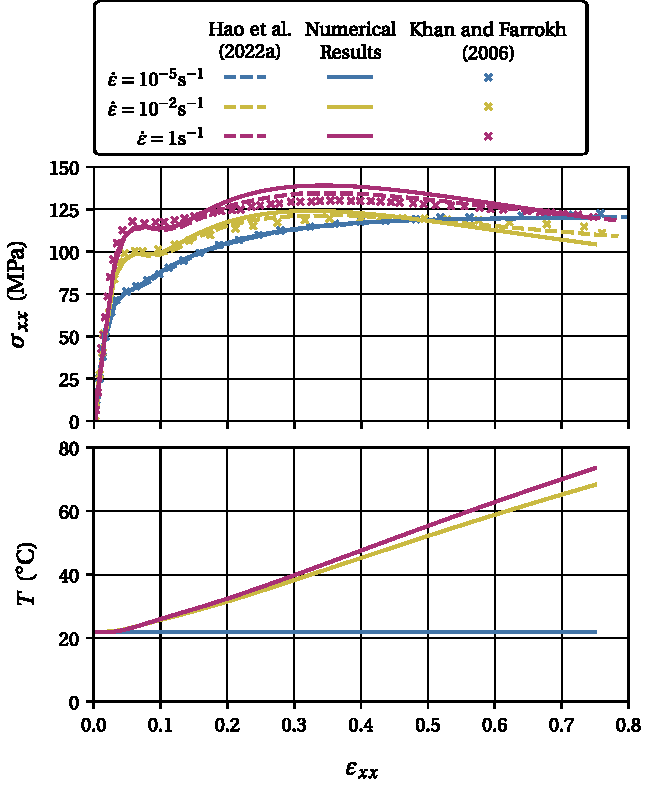
\includegraphics[width=0.85\textwidth]{figures/stress_temp_strain_hao_results}
  \caption{Comparison between the experimental results of \cite{khanThermomechanicalResponseNylon2006}, the numerical results of \cite{haoUnifiedAmorphousCrystalline2022} and the present work for a uniaxial compressive test at strain rates of \SIlist{1e-5;1e-2;1e0}{\per\second}. (a) True strain-true stress curve. (b) True strain-temperature curve.}
\label{fig:stress_temp_strain_hao_results}
\end{figure}

Discussing first the fitness of the model proposed in \cite{haoUnifiedAmorphousCrystalline2022} to describe the experimental results of Khan and Farrokh \citep{khanThermomechanicalResponseNylon2006}, the model captures adequately the elastic range and the first yield point.
As seen from the experimental results, nylon 101 displays double yield, which becomes more noticeable as the rain rate increases.
To the point in Figure~\ref{fig:stress_temp_strain_hao_results}, only the strain rates of \SIlist{1e-2;1e0}{\per\second} show a prominent double yield.
This phenomenon is also correctly described by the model, with a slight underestimation of the stress response for the higher strain rates.
Conversely, regarding the second yield, the model predicts overestimates slightly the stress.

Regarding the implementation and numerical solution found in the present work, for the lowest strain rate considered (\SI{1e-5}{\per\second}), there is perfect agreement with the numerical results presented in \cite{haoUnifiedAmorphousCrystalline2022}.
The same can't be said for the other two strain rates.
Still, until the first yield and subsequent softening ther is good agreement betweeen the two sets of numerical results.
As the strain increases there is a larger descrepency between the two.
There a few reasons for this.
The first concerns mainly the experiment corresponding to a strain rate of \SI{1e-2}{\per\second}, which in the present work as simulated as an adiabatic process.
This is not strictly true and contributes to differences relative to the reference results, which were obtained employing a fully thermomechanical description of the problem including conduction inside the cylinder and converction at its borders.
A further contributing factor, that also affects the response obtained in the present work at \SI{1}{\per\second} is the heterogeneity of the response in the results in \cite{haoUnifiedAmorphousCrystalline2022}.
Despite a homogeneous temperature distribution equal to \SI{71}{\celsius}, the plastic deformation is heterogeneous, breaking the assumptions of the numerical tool employed in this work and further motivating differences in the results obtained.
In general, the implementation developed in this work compares favourably with the one found in \cite{haoUnifiedAmorphousCrystalline2022}.

\subsection{Composite model}

The thermomemechanical problem under analysis consists of the compression of cylinder.
The problem consists of a cylindrical bar of radius $r=\SI{6.413}{\milli\meter}$ and length $h=\SI{53.334}{\milli\meter}$.
The bar is initially at room $T_{0}=T_{\infty}=\SI{295}{\kelvin}$ and is subject to heat transfer by convection at all boundaries, with a heat transfer coefficient $h_{c} = \SI{17.5e-3}{\newton\milli\meter^{-1}\second^{-1}\kelvin^{-1}}$.
The material is modeled by the constitutive model proposed by Hao et al. \citep{hao}, and the material properties are given in Table~\ref{tab:matpropsnecking}.
%
\begin{table}
  \centering
  \caption{Material properties and initial and boundary conditions for the problem concerning the necking of a thermoplastic circular bar.}
  \label{tab:matpropsnecking}
  \begin{tabular}{lccS[exponent-mode=engineering]}
    \hline\hline
    \multicolumn{3}{l}{\textbf{Material Properties}} & {\vphantom{\Big |}Effective value}\\
    \hline
    \vphantom{\Big |}Density & \(\rho\) & (\si{\newton\second^2\milli\meter^{-4}}) & 7.8e-9\\
    \vphantom{\Big |}Bulk modulus & \(\kappa\) & (\si{\newton\milli\meter^{-2}}) & 164206\\
    \vphantom{\Big |}Shear modulus & \(\mu\) & (\si{\newton\milli\meter^{-2}}) & 801938\\
    \vphantom{\Big |}Conductivity & \(k\) & (\si{\newton\second^{-1}\kelvin^{-1}}) & 45\\
    \vphantom{\Big |}Heat capacity & \(C_{\mathbf F}\) & (\si{\milli\meter^2\second^{-2}\kelvin^{-1}}) & 460e6\\
    \vphantom{\Big |}Coefficient of thermal expansion & \(\alpha_T\) & (\si{\kelvin^{-1}}) & 10e-6\\
    \vphantom{\Big |}Dissipation factor & \(\chi\) & (-) & 900e-3\\
    \vphantom{\Big |}Initial yield stress at \(T_0\) & \(\sigma_{y,0}\) & (\si{\newton\milli\meter^{-2}}) & 450\\
    \vphantom{\Big |}Linear hardening coefficient at \(T_0\) & \(H\) & (\si{\newton\milli\meter^{-2}}) & 129.24\\
    \vphantom{\Big |}Saturation exponent & \(\delta\) & (-) & 16.93\\
    \vphantom{\Big |}Saturation yield stress at \(T_0\) & \(\sigma_{y,\infty}\) & (\si{\newton\milli\meter^{-2}}) & 715\\
    \vphantom{\Big |}Thermal softening parameter (\(\sigma_{y,0}\)) & \(\omega_0\) & (\si{\kelvin^{-1}}) & 2e-3\\
    \vphantom{\Big |}Thermal softening parameter (\(\sigma_{u,\infty}, H\)) & \(\omega_h\) & (\si{\kelvin^{-1}}) & 2e-3\\
    \hline
    \multicolumn{3}{l}{\textbf{Boundary Conditions}\vphantom{\Big |}} & \\\hline
    \vphantom{\Big |}Radius of the cylindrical bar & \(r\) & (\si{\milli\meter}) & 6.413\\
    \vphantom{\Big |}Length of the cylindrical bar & \(h\) & (\si{\milli\meter}) & 53.334\\
    \vphantom{\Big |}Maximum displacement at both ends & \(\bar u_y\) & (\si{\milli\meter}) & 8\\
    \vphantom{\Big |}Time to maximum displacement & \(t\) & (\si{\second}) & 8\\
    \vphantom{\Big |}Heat transfer coefficient & \(h_c\) & (\si{\newton\milli\meter^{-1}\kelvin^{-1}}) & 17.5e-3\\
    % \multicolumn{3}{l}{\vphantom{\Big |}All mechanical degrees of freedom fixed in the \(y\)- and \(z\)-directions.}\\
    \hline
    \multicolumn{3}{l}{\textbf{Initial Conditions}\vphantom{\Big |}} & \\\hline
    Initial temperature & \(T_0\) & (\si{\kelvin}) & {293}\\
    \hline
    \multicolumn{3}{l}{\textbf{Reference value} \vphantom{\Big |}} & \\\hline
    \vphantom{\Big |}Temperature at outer radius (\(r\)) & & (\si{\kelvin}) & \\
    \vphantom{\Big |}Longitudinal reaction forces & & (\si{\newton}) & \\
    \hline\hline
  \end{tabular}
\end{table}

Given the restrictions of the tool available for solution only \SI{1e-5}{\per\second} and \SI{1}{\per \second}, corresponding to isothermic and adabatic.
Given the value of the dimensionless parameter.

The results are shown in Figure~\ref{fig:res_hao}
\begin{figure}
  \centering
  \includegraphics[width=0.6\textwidth]{example-image-a}
  \caption{Results hao}
\label{fig:res_hao}
\end{figure}

The results are good
The double yield is captured.
The difference can be interpeted as non homegenouss average lower plastic .


% \section{Wishlist}
%
% Independent variables
% \begin{itemize}
%   \item strain rate, temperature
%   \item stress, temperature
% \end{itemize}
%
% Loading type
% \begin{itemize}
%   \item uniaxial traction
%   \item uniaxial compression
%   \item pure shear
%   \item biaxial traction
%   \item hydrostatic compression
%   \item torsion
% \end{itemize}
%
% time dependency
% \begin{itemize}
%   \item impulse
%   \item constant
%   \item ramp
%   \item harmonic
%   \item cyclic
% \end{itemize}
%
% The most interesting loading schemes are:
% \begin{itemize}
%   \item constant strain rate;
%   \item stress relaxation
%   \item creep
%   \item jump constant strain rate at different strains
%   \item loading unloading
%   \item free shrinkage
% \end{itemize}
%
%
% \section{Constant strain rate experiments}
%
% The experiments employed will be.
%
% Compare yield stresses.
%
% Verify thermal sofetening.
%
% Try and choose polymers above and below the glass transition temperature. Need to model the intrinsic softening.
%
% Check how the initial stiffness varies with the strain rate and the temperature.
%
% \section{Unloading}
%
% Remaining deformation Strobl and friends
%
% \section{Free shrinkage}
%
% Remaining deformation
%
% \section{Heated shrinkage}
%
% \colorbox{CyanBlue}{Try the self healing stuff for fibers.}
%
% \section{Stress relaxation}
%
% Test with stress relaxation, maybe master curve.
%
% \section{Creep}
%
% Test with creep, maybe master curve.
